%!TEX TS-program = xelatex
\documentclass[12pt, a4paper, oneside]{article}

\input{preamble.tex}

% эпиграфы
\usepackage{epigraph}
\setlength\epigraphwidth{.8\textwidth}
\setlength\epigraphrule{0pt}

\usepackage{alltt}

\begin{document}

\section*{Quiz 3: алгоритм обратного распространения ошибки}

\epigraph{Да ладно тебе, Фродо! Хорош ломаться, погнали по фасту сгоняем в Мордор. Туда и обратно, приключение чисто на 20 минут.}{Гендальф Серый (Властелин колец: Братство кольцаб 2001)}

\vspace{-0.5cm}
\subsection*{[2] Задание 1}
\vspace{-0.5cm}

Кратко опишите в чём заключается смысл алгоритма обратного распространения ошибки. Не надо расписывать алгоритм целиком. Вам предстоит сделать это в следующем задании.

\vspace{-0.5cm}
\subsection*{[8] Задание 2}
\vspace{-0.5cm}

Гендальф решает задачу регрессии с помощью нейросети:

\begin{center}
    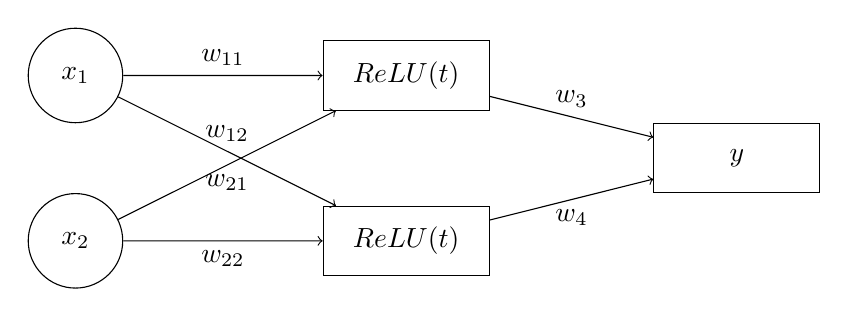
\begin{tikzpicture}[scale=1.4]
        \tikzstyle{place}=[circle, draw=black, minimum size = 12mm]
        \tikzstyle{placeh}=[draw=black, minimum height=25pt,minimum width=60pt,inner sep=2pt]
        
        % Input
        \foreach \x in {1,...,2}
        \draw node at (0, -\x*1.5) [place] (first_\x) {$x_\x$};
        
        % Hidden 1
        \foreach \x in {1,...,2}
        \node at (3, -\x*1.5) [placeh] (second_\x){$ReLU(t)$};     
        
        % Output
        \node at (6, -2.25) [placeh] (fourth){$y$};
        
        \draw [->]  (first_1) to node[above]{$w_{11}$} (second_1);
        \draw [->]  (first_1) to node[above]{$w_{12}$} (second_2);
        \draw [->]  (first_2) to node[below]{$w_{21}$} (second_1);
        \draw [->]  (first_2) to node[below]{$w_{22}$} (second_2);

        \draw [->]  (second_1) to node[above]{$w_3$} (fourth);
        \draw [->]  (second_2) to node[below]{$w_4$} (fourth);
    \end{tikzpicture}
\end{center} 

Помогите Гендальфу сделать два шага стохастического градиентного спуска, используя алгоритм обратного распространения ошибки. У него есть два наблюдения: 

\begin{center}
    \begin{tabular}{cccc} 
        № & $x_1$ & $x_2$ & $y$ \\ \hline 
        1 & $2$ & $-1$ & $-1$ \\ 
        2 & $-1$ & $2$ & $1$ \\ \hline 
    \end{tabular}
\end{center}

Скорость обучения $\gamma = 1$. В качестве инициализации взяты единичные веса. Сначала берётся второе наблюдение, затем первое.

\vspace{-0.5cm}
\subsection*{[0.1] Задание 3}
\vspace{-0.5cm}

Опишите свой любимый момент из режиссерской версии Властелина Колец. Не смотрели? Сомневаюсь, что у вас за этот курс будет хорошая оценка... Исправьте это немедленно. 


\end{document}